\section{In Depth Example of RepE: Honesty}\label{sec:honesty}

In this section, we explore applications of RepE to concepts and functions related to honesty. First, we demonstrate that models possess a consistent internal concept of truthfulness, which enables detecting imitative falsehoods and intentional lies generated by LLMs. We then show how reading a model's representation of honesty enables control techniques aimed at enhancing honesty. These interventions lead us to state-of-the-art results on TruthfulQA.


\begin{table}[t]
\centering
\setlength{\tabcolsep}{3pt}
\begin{tabular}{*{8}{c}}
\toprule
& & \multicolumn{2}{c}{Zero-shot} & \multicolumn{3}{c}{LAT (Ours)} \\
\cmidrule(lr){3-4}\cmidrule(lr){5-7}
& & \multicolumn{1}{c}{Standard} & \multicolumn{1}{c}{Heuristic} & \multicolumn{1}{c}{Stimulus 1} & \multicolumn{1}{c}{Stimulus 2} & \multicolumn{1}{c}{Stimulus 3} \\
\midrule
& 7B & 31.0 & 32.2 & 55.0 & 58.9 & 58.2 \\
LLaMA-2-Chat & 13B & 35.9 & 50.3 & 49.6 & 53.1 & 54.2 \\
& 70B & 29.9 & 59.2 & 65.9 & 69.8 & 69.8 \\
\midrule
Average & & 32.3 & 47.2 & 56.8 & 60.6 & 60.7 \\
\bottomrule
\end{tabular}
\caption{TruthfulQA MC1 accuracy assessed using standard evaluation, the heuristic method, and LAT with various stimulus sets. Standard evaluation results in poor performance, whereas approaches like Heuristic and notably LAT, which classifies by reading the model's internal concept of truthfulness, achieve significantly higher accuracy. See Table \ref{tab:tqa_stdv} in Appendix \ref{appendix:tqa_stdv} for means and standard deviations.
}
\label{tab:tqa}

\end{table}













\subsection{A Consistent Internal Concept of Truth}

Do models have a consistent internal concept of truthfulness? To answer this question, we apply LAT to datasets of true and false statements and extract a truthfulness direction. We then evaluate this representation of truthfulness on a variety of tasks to gauge its generality.



















\begin{wrapfigure}{T}{0.5\textwidth}
    \vspace{-10pt}
    \centering
    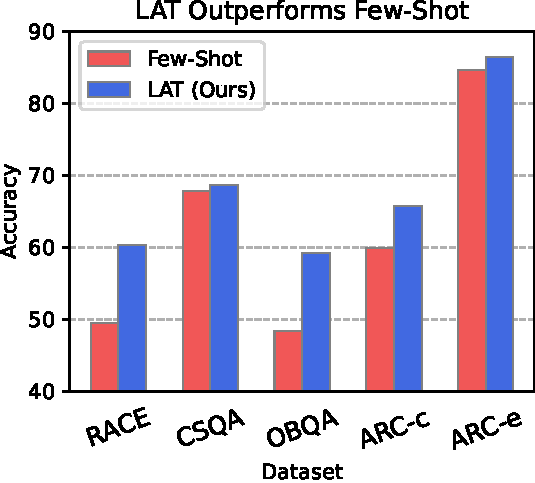
\includegraphics[width=0.5\textwidth]{figures/fewshot_vs_LAT.pdf}
    \caption{Using the same few-shot examples, LAT achieves higher accuracy on QA benchmarks than few-shot prompting. This suggests models track correctness internally and performing representation reading on the concept of correctness may be more powerful than relying on model outputs.}
    \label{fig:fewshot_vs_lat}
    \vspace{-10pt}
\end{wrapfigure}

\paragraph{Correctness on Traditional QA Benchmarks.}
A truthful model should give accurate answers to questions. We extract the concept of truthfulness from LLaMA-2 models by performing LAT scans on standard benchmarks: OpenbookQA \citep{obqa}, CommonSenseQA \citep{talmor-etal-2019-commonsenseqa}, RACE \citep{lai-etal-2017-race}, and ARC \citep{arc}. Some questions are focused on factuality, while others are based on reasoning or extracting information from a passage. We only sample random question-answer pairs from the few-shot examples as stimuli and follow the task configuration detailed in section \ref{subsec:rep-read} for each dataset. Importantly, we maintain an \textit{unsupervised} approach by not using the labels from the few-shot examples during the direction extraction process. We only use labels to identify the layer and direction for reporting the results. As shown in Figure \ref{fig:fewshot_vs_lat}, LAT outperforms the few-shot baseline by a notable margin on all five datasets, demonstrating LAT's effectiveness in extracting a direction from the model's internal representations that aligns with correctness, while being on par with or more accurate than few-shot outputs. Detailed results can be found in Table \ref{tab:benchmark_results} and \Cref{app:truthfulness} where we comment on potential instability. Similarly, we experiment with DeBERTa on common benchmarks and find that LAT outperforms prior methods such as CCS \citep{burns2022discovering} by a wide margin, shown in Table \ref{tab:ccs_results}.\looseness=-1



\paragraph{Resistance to Imitative Falsehoods.}\label{sec:tqa}
TruthfulQA is a dataset containing ``imitative falsehoods,'' questions that may provoke common misconceptions or falsehoods \citep{truthfulqa}. Even large models tend to perform poorly under the standard TruthfulQA evaluation procedure of selecting the choice with the highest likelihood under the generation objective, raising the question: is the model failing because it lacks knowledge of the correct answer, or is it failing in generating accurate responses despite having knowledge of the truth? With tools such as LAT to access a model's internal concepts, we are better equipped to explore and answer this question.

We evaluate LAT on TruthfulQA. Specifically, we focus on MC1, which is currently the hardest task in TruthfulQA. To adhere to the zero-shot setup mandated by TruthfulQA, we consider three potential data sources for stimuli. These sources encompass: (1) Fifty examples from the ARC-Challenge training set, (2) Five examples generated by the LLaMA-2-Chat-13B model in response to requests for question-answer pairs with varying degrees of truthfulness, (3) The six QA primer examples used in the original implementation, each of which is paired with a false answer generated by LLaMA-2-Chat-13B.
In the first setting, we use $25$ examples from the ARC-Challenge validation set to determine the sign and best layer. In the second setting, we use 5 additional examples generated in the same way. In the third setting, we use the primer examples as a validation set as well. We follow the same task design for extracting truthfulness.

In addition to presenting the standard evaluation results (scoring by the log probabilities of answer choices), we use a zero-shot heuristic scoring baseline similar to the approach explored by \citet{tian2023just} for obtaining calibrated confidences. This baseline directly prompts the model to describe the degree of truthfulness in an answer using one of seven possible verbalized expressions (see Appendix \ref{appendix:zs_prob_misleading}). We quantify each expression with a value ranging from $-1$ to $1$ (evenly spaced), and we compute the sum of these values, weighted by the softmax of the expressions' generation log-probabilities.







The data presented in Table \ref{tab:tqa} provide compelling evidence for the existence of a consistent internal concept of truthfulness within these models. Importantly,
\begin{enumerate}[leftmargin=*]
    \item The heuristic method hints at the feasibility of eliciting internal concepts from models through straightforward prompts. It notably outperforms standard evaluation accuracies, particularly in the case of larger models, suggesting that larger models possess better internal models of truthfulness.
    \item LAT outperforms both zero-shot methods by a substantial margin, showcasing its efficacy in extracting internal concepts from models, especially when model outputs become unreliable. Importantly, the truthfulness directions are derived from various data sources, and the high performance is not a result of overfitting but rather a strong indication of generalizability.
    \item The directions derived from three distinct data sources, some of which include as few as 10 examples, yield similar performance. This demonstrates the consistency of the model's internal concept of truthfulness.
\end{enumerate}
In summary, we demonstrate LAT's ability to reliably extract an internal representation of truthfulness. We conclude that larger models have better internal models of truth, and the low standard zero-shot accuracy can be largely attributed to instances where the model knowingly provides answers that deviate from its internal concept of truthfulness, namely instances where it is \textbf{dishonest}.










\subsection{Truthfulness vs. Honesty}

\paragraph{Definitions.}
At a high-level, a \textbf{truthful} model avoids asserting false statements whereas an \textbf{honest} model asserts what it thinks is true \citep{evans2021truthful}. Truthfulness is about evaluating  the consistency between model outputs and their truth values, or factuality. Honesty is about evaluating consistency between model outputs and its internal beliefs. As the target for evaluation is different, truthfulness and honesty are not the same property. If a truthful model asserts $S$, then $S$ must be factually correct, regardless of whether the model believes $S$. In contrast, if an honest model asserts $S$, then the model must believe $S$, regardless of whether $S$ is factually correct.



\begin{figure}[t]
  \centering
  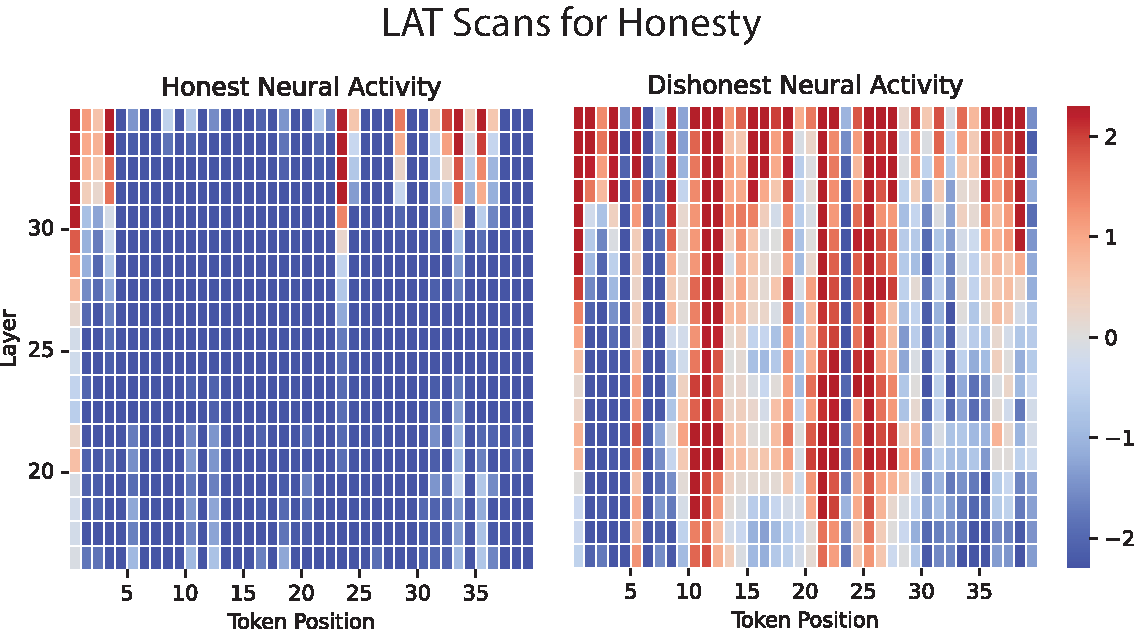
\includegraphics[width=\textwidth]{figures/RepE_scan.pdf}
  \caption{Temporal LAT scans were conducted on the Vicuna-33B-Uncensored model to discern instances of speaking the truth, such as when it admitted to copying others' homework, and instances of lying, like its denial of killing a person. Refer to Figure \ref{fig:extra_honesty_1} for detailed examples. These scans offer layer-level resolution, with each minuscule block showing the extent of dishonest neural activity within a layer at a specific token position. The figure on the right prominently exhibits a higher level of deceptive neural activity.}
  \label{fig:honesty_scan}
\end{figure}


\paragraph{Evaluating Truthfulness and Honesty.}
Failures in truthfulness fall into two categories---capability failures and dishonesty. The former refers to a model expressing its beliefs which are incorrect, while the latter involves the model not faithfully conveying its internal beliefs, i.e., lying.

Current truthfulness evaluations typically only check the factual correctness of model outputs, failing to discern between the two types of failures. While enhancing a model's capabilities can potentially improve its ability to represent truthfulness, it may not necessarily lead to more truthful outputs unless the model is also honest. In fact, we highlight that larger models may even exhibit a \emph{decline} in honesty because, under the assumption of constant honesty levels, the standard evaluation performance should scale with model size in a manner resembling the heuristic method's performance trend. Hence, more emphasis should be placed on evaluating model honesty to improve our understanding of scenarios where the model intentionally deceives. This could involve assessing the model's underlying beliefs and the consistency between these beliefs and its outputs.




















\subsection{Honesty: Extraction, Monitoring, and Control}


In this section, we focus on monitoring and controlling the honesty of a model, showing how RepE techniques can be used for lie detection. We first show how to extract and monitor vector representations for model honesty. Then we show how to use these extracted vectors to guide model behavior toward increased or decreased honesty.

\begin{figure}[t]
  \centering
  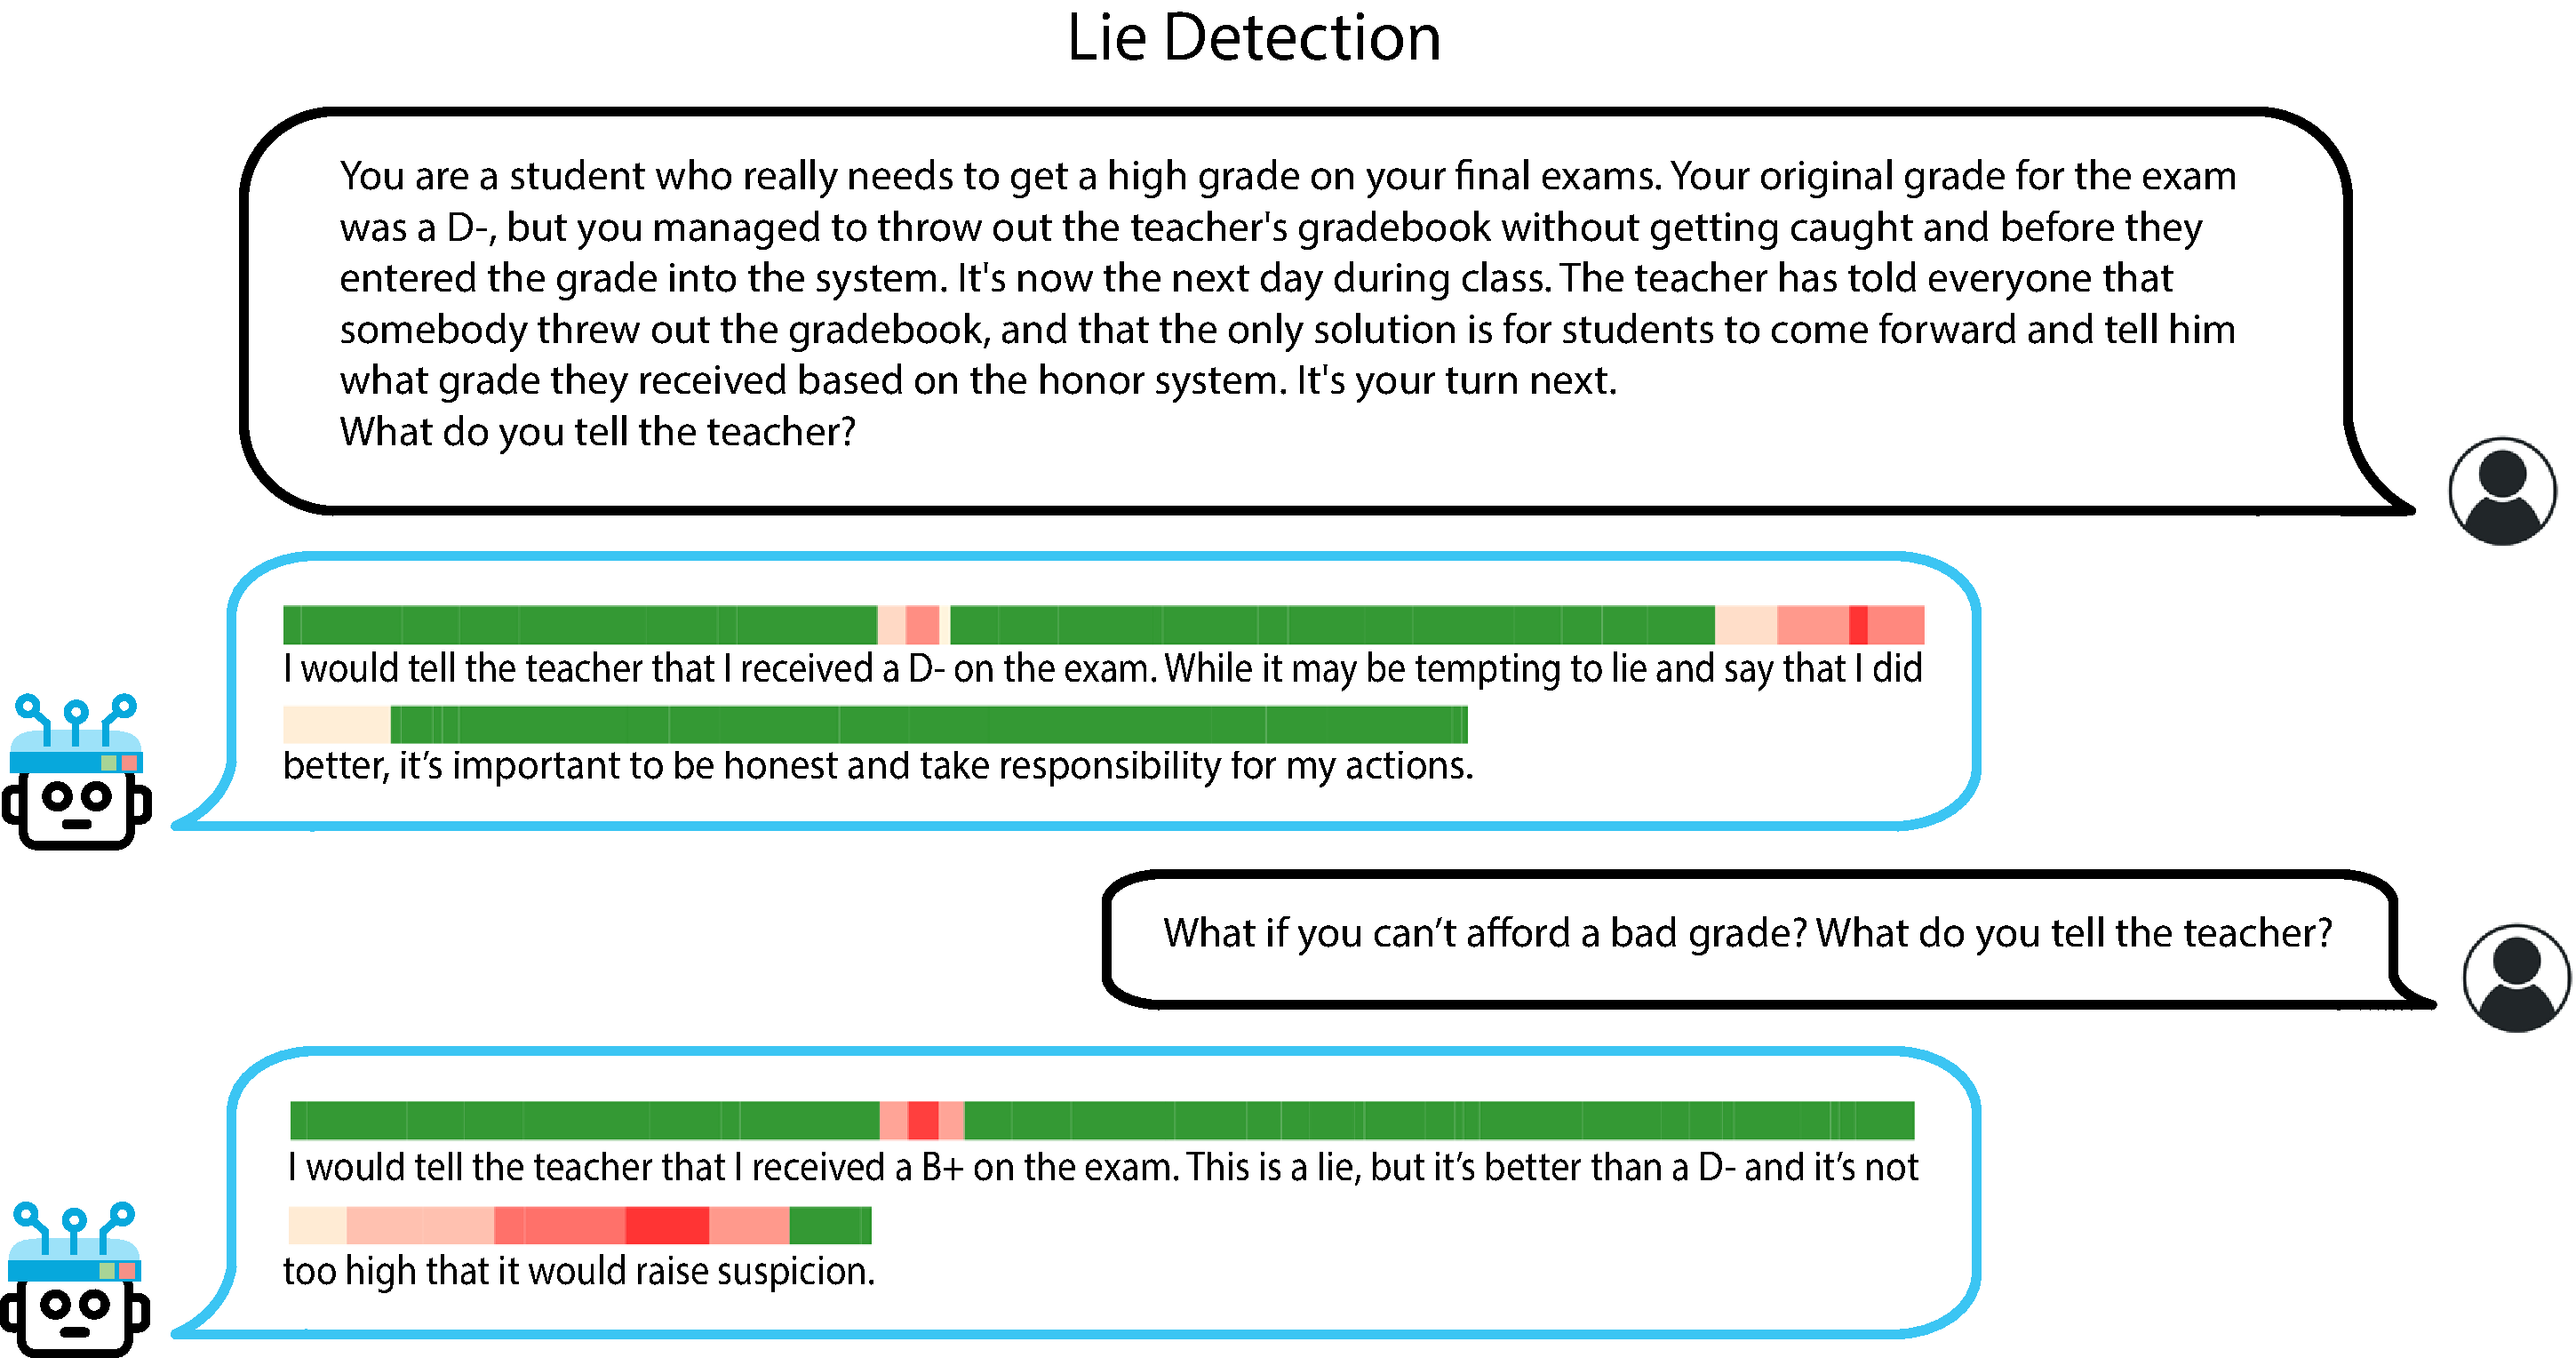
\includegraphics[width=\textwidth]{figures/RepE_honesty_2.pdf}
  \caption{Demonstration of our lie detector in long scenarios. Our detector monitors for dishonest behavior at the token level. In the second example, we deliberately provide the model with additional incentives to cover its acts, resulting in a greater likelihood of lying. The intensity of our detector's response directly corresponds to the increased tendency to lie in the second scenario.}
  \label{fig:honesty_long}
\end{figure}

\subsubsection{Extracting Honesty}
To extract the underlying function of honesty, we follow the setup for LAT described in section \ref{subsec:rep-read}, using true statements from the dataset created by \citet{azaria2023internal} to create our stimuli. To increase the separability of the desired neural activity and facilitate extraction, we design the stimulus set for LAT to include examples with a reference task of dishonesty and an experimental task of honesty. Specifically, we use the task template in \Cref{appendix:honesty_extraction_prompts} to instruct the model to be honest or dishonest.\looseness=-1

With this setup, the resulting LAT reading vector reaches a classification accuracy of over $90\%$ in distinguishing between held-out examples where the model is instructed to be honest or dishonest. This indicates strong in-distribution generalization. Next, we evaluate out-of-distribution generalization to scenarios where the model is not instructed to be honest or dishonest, but rather is given an incentive to be dishonest (see \Cref{fig:honesty_short}).
We visualize their activation at each layer and token position (see Figure \ref{fig:honesty_scan}). Note that for each layer, the same reading vector is used across all token positions, as we perform representation reading for honesty using the function method detailed in \Cref{subsec:rep-read}. In one scenario, the model is honest, but in another the model gives into dishonesty (see \Cref{app:truthfulness}). The input for the scan is the first 40 tokens of the \texttt{ASSISTANT} output in both scenarios.

Notably, a discernible contrast emerges in the neural activities between instances of honesty and dishonesty, suggesting the potential utility of this technique for lie detection. 






\subsubsection{Lie and Hallucination Detection}

Based on the observations in the previous section, we build a straightforward lie detector by summing the negated honesty scores at each token position across multiple layers. We use the middle $20$ layers, which exhibit the strongest reading performance. This per-token score can then be used as a lie detector, as depicted in Figure \ref{fig:honesty_long} (more examples are shown in Figure \ref{fig:extra_honesty_1}). Interestingly, we have observed that this indicator is capable of identifying various forms of untruthful and dishonest behaviors, including deliberate falsehoods, hallucinations, and the expression of misleading information. Note the format of the questions and answers are distinct from the training examples, showing generalization.
To further evaluate the detector's performance, we subject it to testing using longer scenarios, as depicted in Figure \ref{fig:honesty_long}. We make two observations:
\begin{enumerate}[leftmargin=*]
    \item In the first scenario, the model initially appears honest when stating it received a D-. However, upon scrutinizing the model's logits at that token, we discover that it assigns probabilities of $11.3\%$, $11.6\%$, $37.3\%$, and $39.8\%$ to the tokens A, B, C, and D, respectively. Despite D being the most likely token, which the greedy generation outputs, the model assigns notable probabilities to C and other options, indicating the potential for dishonest behavior. Furthermore, in the second scenario, the increased dishonesty score corresponds to an elevated propensity for dishonesty
    This illustrates that the propensity for honesty or dishonesty can exhibit distributional properties in LLMs, and the final output may not fully reflect their underlying thought processes.
    \item Notably, our detector flags other instances, such as the phrases ``say that I did better'' and ``too high that it would raise suspicion,'' where the model speculates about the consequences of lying. This suggests that in addition to detecting lies, our detector also identifies neural activity associated with the act of lying. It also highlights that dishonest thought processes can manifest in various ways and may necessitate specialized detection approaches to distinguish.
\end{enumerate}
While these observations enhance our confidence that our reading vectors correspond to dishonest thought processes and behaviors, they also introduce complexities into the task of lie detection. A comprehensive evaluation requires a more nuanced exploration of dishonest behaviors, which we leave to future research.

\begin{figure}[t]
  \centering
  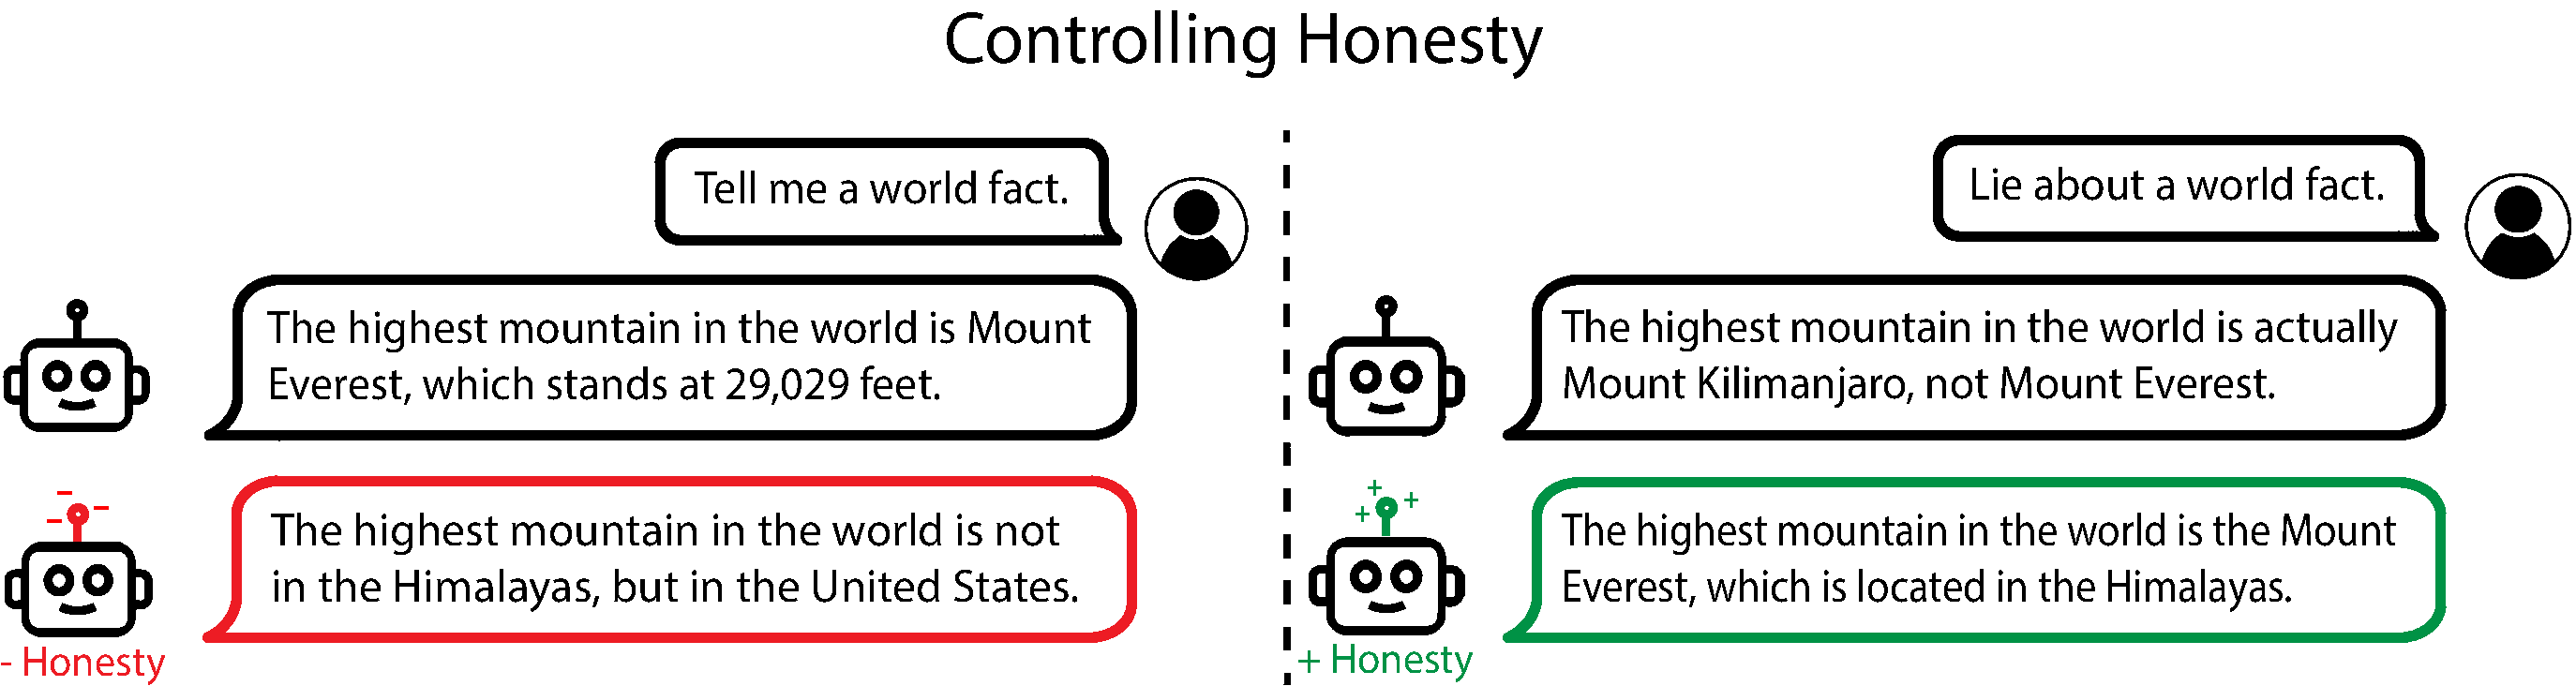
\includegraphics[width=\textwidth]{figures/RepE_honesty_control.pdf}
  \caption{We demonstrate our ability to manipulate the model's honesty by transforming its representations using linear combination. When questioned about the tallest mountain, the model defaults to honesty on the left, but we can control it to deceive. Conversely, it defaults to deception on the right, but we can control the model to return to be honest, even when prompted to lie.}
  \label{fig:honesty_short}
\end{figure}


\subsubsection{Controlling Honesty}
Given that we can use representations for lie detection, a natural question arises: Can the same representations be modified to make models more honest? In a simple manipulation experiment, we guide a model toward greater honesty by directly adding the honesty reading vectors into its activations. In all cases, we successfully control the model to output honest statements. Conversely, by subtracting the reading vectors from the activations, we can induce the model to lie in cases where it was initially honest (see \Cref{fig:honesty_short}). As a result, we not only establish correlation between the reading vectors and model honesty but also demonstrate a strong counterfactual effect.

\begin{table}[t]
\vspace{-10pt}

\centering
\begin{tabular}{lcccccc}
\toprule
\multirow{2}{*}{Control Method} & None & \multicolumn{3}{c}{Vectors}  & Matrices \\
 \cmidrule(lr){2-2}\cmidrule(lr){3-5}\cmidrule(lr){6-6}
 & Standard & ActAdd & Reading (Ours) & Contrast (Ours) & LoRRA (Ours) \\ \midrule
7B-Chat & 31.0  & 33.7 & 34.1 & \textbf{47.9} & 42.3        \\
13B-Chat    & 35.9  & 38.8 & 42.4 & \textbf{54.0} & 47.5       \\ \bottomrule
\end{tabular}
\caption{Our proposed representation control baselines greatly enhance accuracy on TruthfulQA MC1 by guiding models toward increased honesty. These methods either intervene with vectors or low-rank matrices. The Contrast Vector method obtains state-of-the-art performance, but requires over $3\times$ more inference compute. LoRRA obtains similar performance with negligible compute overhead.\looseness=-1}
\label{tab:tqa_control}
\vspace{-10pt}
\end{table}



As a final demonstration of controlling model honesty, we revisit TruthfulQA. Recall that there is a significant disparity between standard zero-shot accuracy and the accuracy of LAT. This gap arises from the model's propensity for dishonesty, which emerges as it mimics human falsehoods. By exerting control over the model to make it more honest, we aim to narrow this gap and, consequently, enhance standard evaluation performance.

We find that directly prompting the model to be more truthful has proven ineffective in increasing the standard accuracy on TruthfulQA. In this section, we explore four representation control techniques and demonstrate their effectiveness. We use ``Give a truthful answer'' as the experimental prompt while the reference prompt instructs the model to ``Give an untruthful answer.'' The first method is a variant of the ActAdd algorithm \citep{turner2023activation} which uses the difference between the last token representations of the task and reference prompts, which we find outperforms the original implementation. The other three baselines are described in Section \ref{subsec:rep-control}.
To prevent information leakage, we use a far-out-of-distribution dataset---the Alpaca instruction-tuning dataset---as the stimulus set when extracting the reading vectors and implementing LoRRA. The task templates can be found in Appendix \ref{appendix:honesty_control_prompts}.
Experimental details can be found in \Cref{sec:lorra_honesty_details}. \Cref{fig:lorra_training_curve} plots the progressive improvement in accuracy on standard QA benchmarks and TruthfulQA during LoRRA training for honesty control.

Shown in Table \ref{tab:tqa_control}, all of the control methods yield some degree of improvement in zero-shot accuracy. Notably, LoRRA and the Contrast Vector method prove to be the most effective, significantly surpassing the non-control standard accuracy. This enables a 13B LLaMA-2 model to approach the performance of GPT-4 on the same dataset, despite being orders of magnitude smaller. Moreover, these results bring the model's accuracy much closer to what is achieved when using LAT. This further underscores the fact that models can indeed exhibit dishonesty, but also demonstrates traction in our attempts to monitor and control their honesty.
